% !TeX root = ../../thesis.tex

\section{\acs{UEFI} Shell}

Part of the family of \ac{UEFI} specifications is a shell specification that defines a feature\-/rich \ac{UEFI} shell application to interact with the \ac{UEFI} environment \cite[Section 1.1]{uefi-shell-spec}.
It offers commands relating to boot and general configuration, device and driver management, file system access, networking \cite[Section 5.1]{uefi-shell-spec}, and scripting \cite[Section 4]{uefi-shell-spec}.
A shell application may already be part of the boot options but can always be supplied in the default boot path of removable media.

The \ac{UEFI} shell is a great tool to visualize the \ac{UEFI} environment.
With the \program{devtree} command, for example, we can see the tree of all handles complying with the \ac{UEFI} driver model.
This also serves as a great reference on how \hyperref[lst:device-path-protocol]{device paths} are formed.
\autoref{fig:devtree} shows the output of \program{devtree} cropped to show a \ac{GPT} formatted hard drive and its logical partitions.
When the firmware discovers a block device it is also required to search for a partition table and create a device handle for each partition.
Device drivers abstracting file systems can then be connected to a partition handle and check whether a supported file system format type is present.
The first partition listed in \autoref{fig:devtree} as a \emph{FAT File System} is the \ac{ESP} of this drive.

\begin{figure}[htb]
    \centering
    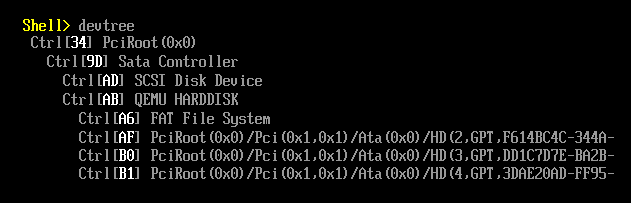
\includegraphics[width=1.0\textwidth]{uefi/devtree}
    \caption{Shortened \ac{UEFI} shell output of \program{devtree}}
    \label{fig:devtree}
\end{figure}

With \program{openinfo} we can see the group of protocols that a handle represents.
\autoref{fig:openinfo} shows the output when querying the handle of an \ac{ESP}.
Since this \ac{ESP} is installed in a logical partition, an instance of the \nameref{lst:partition-information-protocol} is present.
The command also lists the agent handles of each protocol and how the protocol was accessed.
\code{TestProt} is often used in the \code{Supported()} function of a driver, while \code{GetProt} is then used to open the protocol for consumption within the \code{Start()} function.

\begin{figure}[htb]
    \centering
    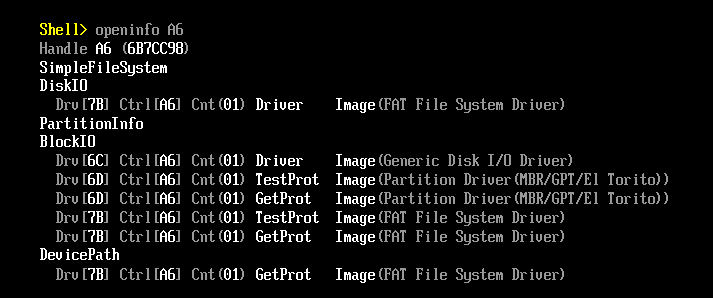
\includegraphics[width=1.0\textwidth]{uefi/openinfo}
    \caption{Shortened \ac{UEFI} shell output of \program{openinfo}}
    \label{fig:openinfo}
\end{figure}